\chapter{Função do Receptor}

\section{Fundamentos Teóricos}

A caracterização prévia das informações contidas no sinal é imprescindível para o processamento. A avaliação da performance e da qualidade dos dados da estações sismográficas foram feitas no software livre PQLX.  A metodologia do PQLX é baseada no trabalho de \cite{McNamara_Buland_2004}. Esse procedimento é bastante usado para se obter a informação espectral sísmica.

No programa PQLX a série temporal é segmentada em intervalos de uma hora, com 50\% de superposição do sinal. Cada janela de hora está separada em 13 intervalos com 75\% de superposição para calcular a “Power Spectral Density”. As médias obtidas para cada um dos 13 intervalos são usadas para estimar a “Probability Density Functions”, calculados a partir das médias pelo número total de segmentos de hora em hora. 

Essa metodologia de \cite{McNamara_Buland_2004} difere dos métodos habitualmente utilizados, porque não é necessário a visualização de todo conjunto de dados para uma estima qualitativa do sinal, observado na Figura \ref{PQLX}.

\begin{figure}[!ht]
\centering
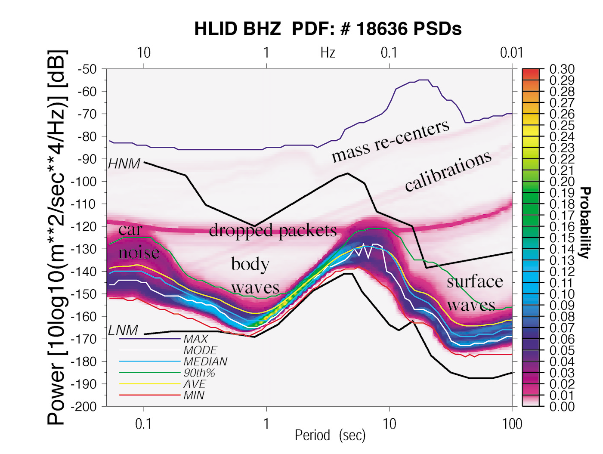
\includegraphics[scale=0.8]{mcnamura_buland.png}
\caption{Análise qualitativa do sinal atraves das \textit{Power Density Functions}. \cite{McNamara_Buland_2004} }
\label{PQLX}
\end{figure}

A garantia da fiabilidade do tempo de chegada da onda P é fundamental para o processamento gerar resultados consistentes. Portanto testes com o tempo de chegada da onda P forão feitos. \cite{gibbons_identification_2006} mostra que fazendo a correlação de dois eventos distantes em uma estação sismográfica consegue-se caracterizar esse tempo de chegada, como é visto na Figura \ref{teste_tempo}. \cite{gibbons_identification_2006} assume que  se não há alterações mensuráveis na velocidade da estrutura entre a fonte e os receptores, ondas sísmicas de dois eventos co-localizados terá a mesma duração de tempo para chegar a um determinado sensor. A função de correlação cruzada para um dado sinal a uma dada estação mede que a semelhança entre a porção posterior do sismograma é a do modelo de forma de onda. O tempo de separação entre o início do modelo e o valor máximo da função de correlação cruzada deve ser igual ao tempo que separa os dois tempos de origem dos eventos para todas as estações. Qualquer discrepância nos tempos de separação medido em duas estações diferentes, o que não é atribuível a diferença entre fontes ou uma SNR baixa, deve ser o resultado de uma anomalia em sincronismo um, ou ambos, dos instrumentos.

Nesste trabalho utilizamos uma metodologia semelhante a de \cite{gibbons_identification_2006}. Utilizou-se um sismo distante de um par de estações sismográficas próximas. Com os sinais registrados fez-se a correlação cruzada dos dados. Como a fonte está distante das estações a correlação dos sinais deve ser próxima de zero. Este teste do tempo de chegada da onda P é para garantir a confiabilidade dos dados das estações temporárias. Portanto em cada par de estações correlacionadas sempre tinha uma estação permanente, estação com dados confiáveis.

\begin{figure}[!ht]
\centering
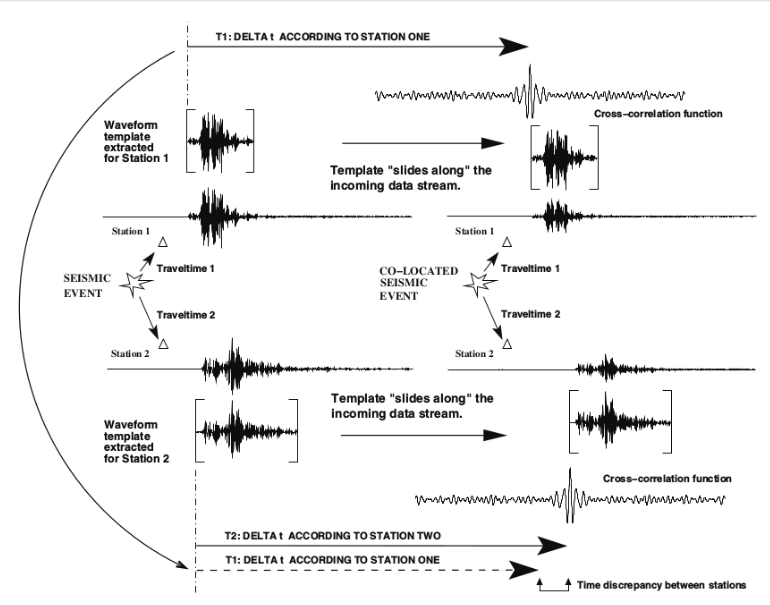
\includegraphics[scale=0.6]{correlacao_tempo_de_chegada.png}
\caption{Uma ilustração esquemática de como dois eventos sucessivos de fontes sísmicas quase idênticas que podem ser explorados para revelar anomalias dos tempo de chegada da onda P numa dada estação. \citep{gibbons_identification_2006}}
\label{teste_tempo}
\end{figure}

No ínicio desse trabalho somente os dados de eventos incluídos no catálogo do IRIS (\textit{Incorporated Research Institutions for Seismology}) com magnitude maior que 5,5 entre maio de 2011 e maio de 2012 foram utilizados. Porém agora utiliza-se dados coletados na rede Sismográfica, mostrada na \ref{map_loc}, até o fim do segundo semestre de 2013. A Figura \ref{mapa_eventos} mostra eventos sísmicos registrados na estação STA08 mostrando a delimitação dos eventos pela distância epicentral, além de mostrar sismos com magnitude maior que 5.5 mb.

O sismômetro registra pequenas variações horizontais e verticais de amplitude das partículas do terreno na escala microscópica ao longo das direções Vertical (Z), Norte-Sul (N) e Leste-Oeste (E), chamado sistema ZNE, como observado na Figura \ref{simograma}. No entanto, o sinal bruto nas direções ZNE não está alinhado aos eixos de propagação das ondas geradas pelo sismo, logo a resposta em cada componente mostra uma sobreposição de vários tipos de ondas. Com a finalidade de isolar a contribuição de cada onda registrada nos dados, o sistema de coordenadas dos registros são rotacionadas, através do SAC (\textit{Seismic Analysis Code}), para se alinharem com os eixos de propagação das ondas através da seguinte matriz de rotação:

\begin{eqnarray} \label{rotação}
\left[ \begin{array}{c} R \\ T \\ Z \end{array} \right] = \begin{bmatrix} \cos \theta & \sin \theta & 0 \\ - \sin \theta & \cos \theta & 0 \\ 0 & 0 & 1 \end{bmatrix} \left[ \begin{array}{c} E \\ N \\ Z \end{array} \right]
\end{eqnarray}


O resultado da equação \ref{rotação} discrimina claramente a contribuição de cada componente  no sismograma. A componente N (norte-sul) transforma-se na componente T (transversal) e guarda os registro da componente horizontal da onda S, chamada de onda SH. A resposta da onda SV é resgistrada na componente radial do sismograma, chamada R, como pode ser visualizada na Figura \ref{sismo_radial}.   

\begin{figure}[!ht]
\centering
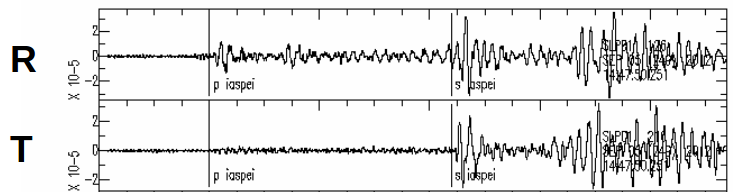
\includegraphics[scale=0.6]{Componente_Radial_Transversal.png}
\caption{Sismograma mostrando as componentes Radial e Transversal.}
\label{sismo_radial}
\end{figure}

Para o cálculo a espessura crustal na região utilizou-se o método da Função do Receptor, que foi desenvolvido por \cite{Langston_1977}. O programa SAC (\textit{Seismic Analysis Code}) foi usado para fazer o processamento e o cálculo das Funções Receptores. Tal método faz uso do sinal de tele-sismos, geradores de ondas planas de incidência quase-vertical embaixo de uma dada estação. A onda P incide na discontinuidade de Mohorovicic e se decompõe em uma onda P transmitida e uma onda S convertida. A diferença do tempo de chegada das duas ondas, onda S tem velocidade inferior a onda P, e de outras reflexões permite inferir a profundidade da discontinuidade de Mohorovicic, também chamada de Moho, como mostrado na Figura \ref{funcoes_sinteticas} .

\begin{figure}[!ht]
\centering
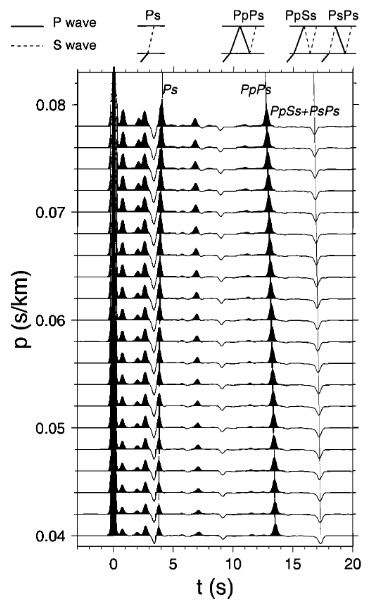
\includegraphics[scale=0.8]{funcoes_sinteticas.png}
\caption{Funções do Receptor em função do parâmetro do raio para o Modelo de Velocidade Padrão do Sul da Califórnia, em \cite{Zhu_Kanamori_2000}. A fase Ps convertida em Moho e suas múltiplas  PpPs, PpSs, e PsPs e seus traços são ilustrados no topo da imagem. Outras reflexões não-rotuladas são as conversões P-S em 5.5 km e 16 km, discontinuidades intracrustais no modelo.}
\label{funcoes_sinteticas}
\end{figure}

Para uma estimativa precisa das Funções do Receptor é essencial que o tempo de chegada da onda P seja determinado com baixa incerteza. Então os dados foram examinados visualmente para registrar o tempo de chegada da onda P direta. 

As Funções do Receptor são calculadas com uma deconvolução componente radial (R) pela componente vertical (Z), como é mostrado por \cite{clayton_source_1976}, \cite{Langston_1977}, \cite{ammon_isolation_1991}, \cite{cassidy_numerical_1992}, \cite{Zhu_Kanamori_2000}. Essa operação remove efetivamente a resposta instrumental, a assinatura da fonte e a propagação da fonte até Moho. E o sinal resultante é a assinatura da propagação próxima à estação. Então a Função do Receptor é sensível na delimitação da estruturação superficial da crosta embaixo da estação.

Computar as Funções do Receptor é um problema de deconvolução,  \cite{ligorria_iterative_1999}. \cite{langston_structure_1979} descreve a resposta do deslocamento teórico para uma onda plana P incidindo sobre uma empilhamento de interfaces horizontais ou inclinadas no domínio do tempo pode ser dada por:

\begin{eqnarray} \label{lang_equacao}
D_{V}(t) = I(t) * S(t) * E_{V}(t)
\nonumber
\\
D_{R}(t) = I(t) * S(t) * E_{R}(t)
\\
\nonumber
D_{T}(t) = I(t) * S(t) * E_{T}(t)
\end{eqnarray}

Onde $S(t)$ é a resposta efetiva da fonte em função do tempo de uma onda incidente, $I(t)$ é a resposta do impulso instrumental e $E_{V}(t)$, $E_{R}(t)$ e $E_{T}(t)$ são as respostas do impulso da estruturua vertical, radial e tangencial, respectivamente. A componente $S(t)$ pode ser muito complicada de ser computada, pois ela é relacionada a história do deslocamento no tempo e reverberações na aŕea da fonte.

\cite{langston_structure_1979} assume que eventos profundos observados em dados telessísmicos, na componente vertical do movimento do terreno ($D_{V}(t)$), se comportam como um pulso em função do tempo convoluído com a resposta instrumental e com chegadas tardias menores. Cálculos teóricos para estruturas crustais mostram que reverberações crustais e fases convertidas na componente vertical de ondas P são menores. Então se aproxima:

\begin{eqnarray} \label{lang_suposicao}
I(t) * S(t) \simeq D_{V}(t)
\end{eqnarray}

\cite{langston_structure_1979} faz uma suposição implícita que $D_{V}(t)$ comporta-se como uma função delta de Dirac, como pode ser observado na equação \ref{lang_suposicao}. Assumindo que a resposta instrumental é compensada entre as componentes, $E_{R}(t)$ e $E_{T}(t)$ podem ser encontrados passando para o domínio da frequência a equação \ref{lang_equacao} e fazendo as seguintes deconvoluções:

\begin{eqnarray} \label{lang_resposta}
E_{R}(\omega) =  \frac{D_{R}(\omega)}{I(\omega)S(\omega)} \simeq \frac{D_{R}(\omega)}{D_{V}(\omega)}
\\ \nonumber
E_{T}(\omega) =  \frac{D_{T}(\omega)}{I(\omega)S(\omega)} \simeq \frac{D_{T}(\omega)}{D_{V}(\omega)}
\end{eqnarray}

$E_{R}(t)$ e $E_{T}(t)$ são retransformadas para o domínio do tempo, importante lembrar que nessa técnica a informação da fase é conservada. \cite{langston_structure_1979} resalta que o resultado da série temporal pode ser interpretado diretamente com um sismograma, permitindo que tempo e amplitude de chegadas possam ser examinadas de uma maneira inequívoca.

\cite{clayton_source_1976}, \cite{langston_structure_1979}, \cite{ligorria_iterative_1999} mostram que o processo de deconvolução possui um instabilidade numérica devido a vários fatores, como o ruído aleatório contido nos dados e a limitação da banda de frequência. Para acabar com os problemas gerados na deconvolução, \cite{clayton_source_1976} introduz um nível de amplitude mínimo permitido da fonte, nomeado de \textit{water-level}, como pode ser visto na Figura Figura \ref{water_level}. Faz-se isso para reduzir componentes de ruídos espúrios e efeitos de pequenos erros na estimação da fonte. Na deconvolução \textit{water-level} a maneira de se evitar a divisão por números pequenos é substituir esses valores pequenos no denominador por uma fração do valor máximo do denominador (para todas as frequências), tal fração é chamada de parâmetro de \textit{water-level}, segundo \cite{Ammon_waterlevel_1997}. \textit{water-level} pode agir, em alguns casos, como um filtro "passa-baixa", "passa-alta" e "não-passa", como mostrado na Figura \ref{water_level} .

\begin{figure}[!ht]
\centering
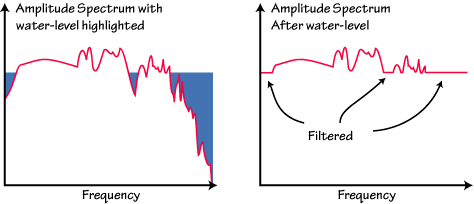
\includegraphics[scale=0.8]{water_level.png}
\caption{Gráficos mostrando o funcionamento do \textit{water-level}, segundo \cite{Ammon_waterlevel_1997}.}
\label{water_level}
\end{figure}

No processamento dos dados a deconvolução no domínio do tempo feita é de acordo com a teoria criada por \cite{ligorria_iterative_1999}, esta é nomeada de deconvolução interativa. Tal método segue a ideia de \cite{kikuchi_inversion_1982}, que é usado para estimar funções do tempo de fontes de grandes terremotos. A deconvolução interativa de  \cite{ligorria_iterative_1999} minimiza através do método dos mínimos quadrados a diferença entre o sismograma horizontal observado e um sinal predito pela convolução de um conjunto de picos atualizados interativamente com a componente vertical do sismograma.

\begin{figure}[!ht]
\centering
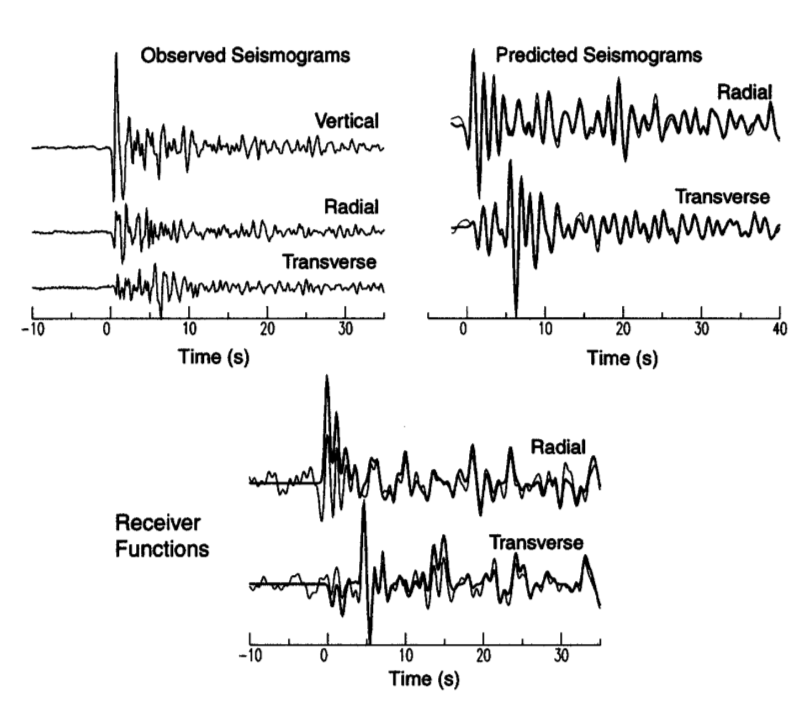
\includegraphics[scale=0.5]{deconvolucao_interativa.png}
\caption{Estimando a Função do Receptor utilizando pequenos períodos. Os sinais originais são mostrados na parte superior esquerda, as funções do Receptor calculadas utilizando \textit{water-level} são comparadas com o método interativo no painel inferior. Os sinais horizontais preditos são comparados com os sinais horizontais observados no painel superior direito. \citep{ligorria_iterative_1999}.}
\label{deconvolucao_interativa}
\end{figure}

\section*{Pós-processamento}

Após gerar sismogramas pela deconvolução Interativa, as séries temporais passaram por um processo de triagem para qualificar as que obtveram melhor resultado. Tal seleção foi feita sob um critério visual observando as funções do receptor que respeitam o formato determinado por \citep{langston_structure_1979}.

Tendo como objetivo a análise da estrutura da crosta, buscou-se inicialmente o cálculo da profundidade de Moho, um importante parâmetro porque é relacionada à geologia e a evolução tectônica da região. \cite{Zhu_Kanamori_2000} propõe um método robusto utilizando a análise das Funções do Receptor para calcular a profundidade de Moho.

Com um modelo da estrutura da Terra, neste caso o IASPEI 91 em \cite{kennet_iaspei_1991}, utiliza as velocidades medianas na crosta para calcular as diferenças de tempo teórica entre a onda P direta e a onda P convertida em S, bem como os tempos das outras reverberações na crosta. De posse de uma dada velocidade $v_{P}$, os tempos de chegada podem ser calculados usando a profundidade de Moho ($H$), a razão $v_{P}$/$v_{S}$ e o parâmetro do raio ($p$), dependente da localização do evento e da profundidade, do modelo.

\cite{Zhu_Kanamori_2000} mostra que os tempos teóricos entre $P_{S}$ e P podem ser utilizados para estimar a espessura crustal, dado uma velocidade crustal média:

\begin{eqnarray}
H = {\frac{t_{P_{s}}}{{\sqrt{\frac{1}{V_{s}^{2}} - p^{2}}} - \sqrt{\frac{1}{V_{p}^{2}} - p^{2}}}}
\end{eqnarray}

E o erro pode ser dado por:

\begin{eqnarray}
\Delta H = \frac{\partial H}{\partial V_{p}} \Delta V_{p}
\end{eqnarray}

Porém a dependência de $t_{Ps}$ em relação a $V_{p}$ não é tão forte quanto a $V_{s}$, especificamente à razão $V_{p}/V_{s}$, $\kappa$. Logo o erro e quantificado:

\begin{eqnarray}
\Delta H = \frac{\partial H}{\partial \kappa } \Delta \kappa 
\end{eqnarray}

\cite{Zhu_Kanamori_2000} demonstra que uma variação de 0.1 na razão $v_{P}$/$v_{S}$ pode acarretar erros de aproximadamente 4 km na espessura crustal. Essa ambiguidade pode ser reduzida utilizando as outras fases, reverberações, da onda P. Tais fases provém informações adicionais, como mostrado nas equações abaixo:

\begin{eqnarray}
H = {\frac{t_{P_{p}P_{s}}}{{\sqrt{\frac{1}{V_{s}^{2}} - p^{2}}} + \sqrt{\frac{1}{V_{p}^{2}} - p^{2}}}}
\end{eqnarray}

\begin{eqnarray}
H = \frac{t_{P_{p}P_{s}+P_{s}P_{s}}}{{2\sqrt{\frac{1}{V_{s}^{2}}- p^{2}}}}
\end{eqnarray}

Em situações reais, identificar a $P_{s}$ em Moho e as múltiplas e medir seus tempos de chegada em um único traço da função do receptor pode ser muito difícil devido ao ruído de fundo, espalhamento devido a heterogeneidades crustais e conversões P para S de outras discontinuidades de velocidades.

Para aumentar a razão sinal/ruído empilha-se as funções do receptor de multiplos eventos. Esse empilhamento é feito no domínio do tempo para um aglomerado de eventos. \cite{Zhu_Kanamori_2000} define um empilhamento $H$-$\kappa$ como:

\begin{eqnarray} \label{Hk_stack}
s(H,\kappa) = \omega_{1}r(t_{1}) + \omega_{2}r(t_{2}) + \omega_{3}r(t_{3})
\end{eqnarray}

onde $r(t)$ é a função do receptor radial, $t_{1}$, $t_{2}$ e $t_{3}$ são os tempos de chegada preditos  $t_{s}$,  $t_{P_{p}P_{s}}$ e  $t_{P_{p}P_{s}+P_{s}P_{s}}$ correspondente a uma espessura crustal $H$ e a uma razão $V_{p}/V_{s}$ e $\omega_{i}$ são os pesos dos fatores, e $\sum \omega_{i} = 1$. 

Ao invés de tentar ajustar toda a função, o método faz uma pesquisa, \textit{grid search}, da espessura crustal e da razão $v_{P}$/$v_{S}$ para calcular o tempo de chegada teórico das ondas P convertidas em S e das múltiplas para cada registro. A melhor combinação da espessura crustal e da razão $v_{P}$/$v_{S}$, $\kappa$, é aquela que maximiza o valor das amplitudes reais das funções receptor, como pode ser visualizado na Figura \ref{grid_search} .

\begin{figure}[!ht]
\centering
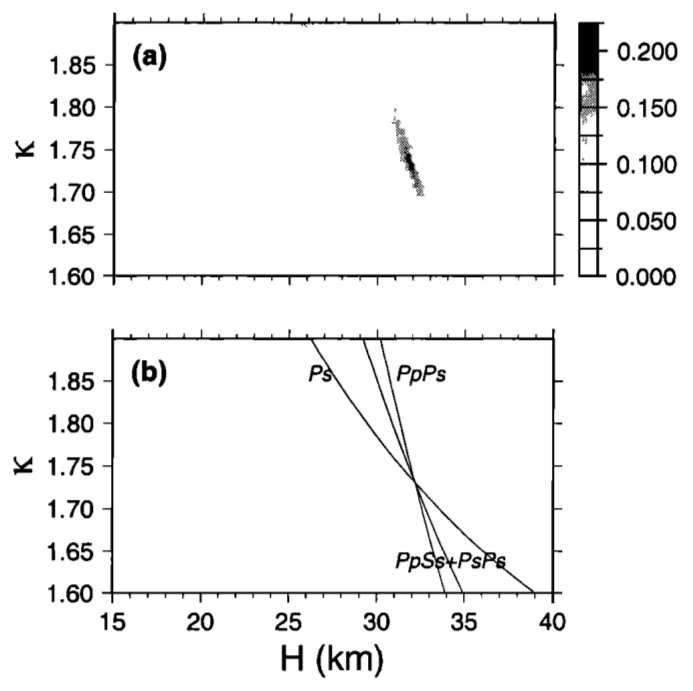
\includegraphics[scale=0.5]{grid_search.png}
\caption{(a) $s(H,\kappa)$ do empilhamento das funções do receptor utilizando a equação \ref{Hk_stack} . Ela encontra o ponto máximo quando se usa uma espessura crustal $H$ e uma razão $v_{P}$/$v_{S}$ coerentes. (b) Relações $H-\kappa$ para diferentes fases convertidas em Moho. Cada curva representa a contribuição dessa fase convertida ao empilhamento, segundo \cite{Zhu_Kanamori_2000}.}
\label{grid_search}
\end{figure}

\cite{julia_deep_2008} mostra uma dependência azimutal das funções do receptor. Para isso ele mostra que separando as funções do receptor de acordo com o backazimute e o parâmetro do raio pode-se checar a variação lateral das estruturas. Os dados são separados em 4 grupos, segundo o azimute entre o sismo e a estação. 
\pagebreak
